\documentclass{beamer}

% Encoding & language
\usepackage[T1]{fontenc}
\usepackage[utf8]{inputenc}
\usepackage[english]{babel}
\usepackage{transparent}

% Bibliography
\usepackage[numbers]{natbib}
\bibliographystyle{ieeetr}

% Figures, tables, colors
\usepackage{graphicx}
\usepackage{subcaption}
\usepackage{tabularx}
\usepackage{booktabs}
\usepackage{multirow}
\usepackage{makecell}
\usepackage[table, svgnames]{xcolor}

\usepackage{caption}
\captionsetup[table]{justification=centering}

% Beamer
\setbeamerfont{framesubtitle}{size=\normalsize}

% Misc
\usepackage{amsmath}
\usepackage{amssymb}
\usepackage{hyperref}
\usepackage{tikz}
\usetikzlibrary{arrows.meta, positioning, calc}
\DeclareMathOperator{\jinc}{jinc}

% Section.slide numbering in frame titles (e.g. "2.3")
\newcounter{sframe}[section]
\renewcommand{\thesframe}{\thesection.\arabic{sframe}}
\newcommand{\ftitle}[1]{\stepcounter{sframe}{\normalsize\thesframe}\quad #1}

% Transparent, Checkmark
\usepackage{transparent}
\newcommand{\dimtxt}[1]{{\transparent{0.25}#1}} % 0.25-0.45
\usepackage{pifont}
\newcommand{\cmark}{\ding{51}}
\newcommand{\xmark}{\ding{55}}

\mode<presentation>{
  \usetheme{Madrid}
  \usecolortheme{default}
  \setbeamertemplate{caption}[numbered]
}

\title[Solar Radio Interferometer Simulation]{%
  {\Large\bfseries End-to-End Simulation of a Four-Element UHF Radio\\
  Interferometer for Solar Radio Observation at 610~MHz}%
}

\subtitle{Graduation Thesis Defense}

\author[N. B. Quan]
{Nguyen Ba Quan (20224350) \\ Supervisor: Assoc.\ Prof.\ Dr.\ Ha Duyen Trung}

\institute[SEEE--HUST]
{
School of Electrical and Electronic Engineering \\
Hanoi University of Science and Technology
}

\date{\today}

\setbeamertemplate{bibliography item}{\insertbiblabel}

\begin{document}

% ============================================================
% Title
\begin{frame}
  \titlepage
\end{frame}

\begin{frame}{Outline}
\tableofcontents
\end{frame}

% ============================================================
\section{Motivation}

\begin{frame}{\ftitle{Problem and Motivation}}
\begin{columns}[c]
\column{.46\textwidth}
\centering
\scriptsize
\colorbox{blue!8}{\parbox{.92\linewidth}{\centering Solar flares \&
coronal mass ejections $\to$ \textbf{solar radio bursts}}}\\[3pt]
$\Downarrow$\\[3pt]
\colorbox{blue!8}{\parbox{.92\linewidth}{\centering Changes the
ionosphere's electron density}}\\[3pt]
$\Downarrow$\\[3pt]
\colorbox{orange!15}{\parbox{.92\linewidth}{\centering Disturbs
electronic devices --- e.g.\ \textbf{2022 Starlink}: 38/49 satellites
lost to a geomagnetic storm~\cite{berger2023starlink}}}\\[3pt]
$\Downarrow$\\[3pt]
\colorbox{green!15}{\parbox{.92\linewidth}{\centering $\Rightarrow$
Ground-based radio observation gives \textbf{1--3 days} of early
warning}}
\column{.5\textwidth}
\centering
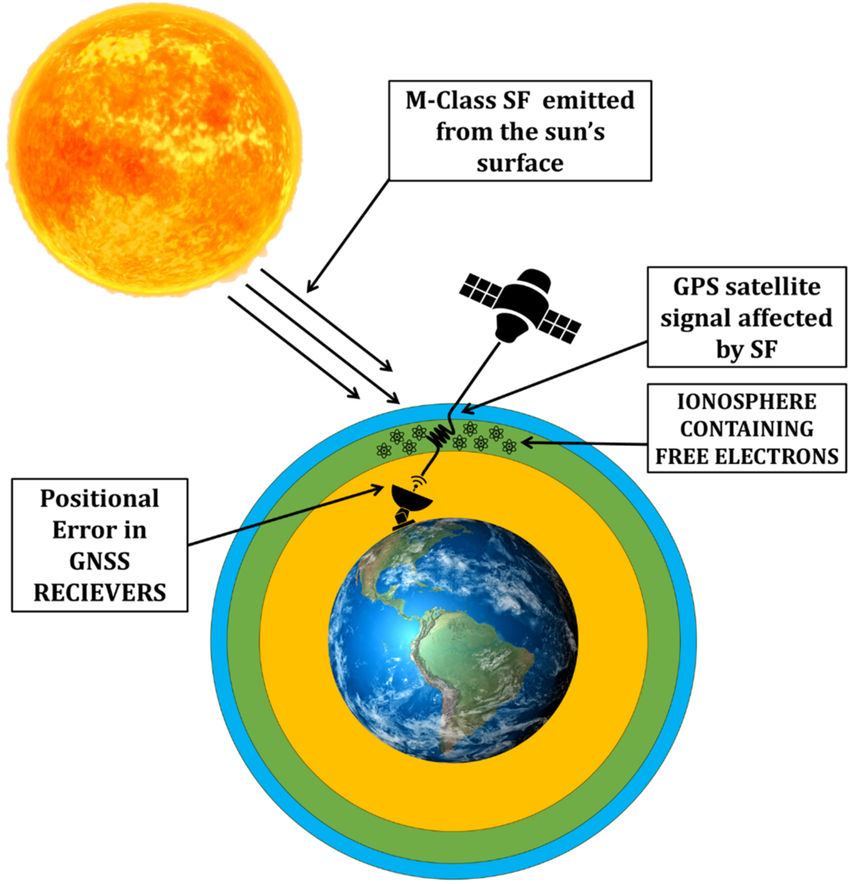
\includegraphics[width=\linewidth]{figs/fig_gnss_ionosphere.png}
\end{columns}
\vspace{4pt}
\centering
\small Fig.~1. How solar radio bursts affect our electronic devices.
\end{frame}

\begin{frame}{\ftitle{Big Dish vs.\ Aperture Synthesis}}
\begin{columns}[t]
\column{.48\textwidth}
\centering
\textbf{Big Parabolic Antenna}\\{\footnotesize (Traditional interferometry)}\\[3pt]
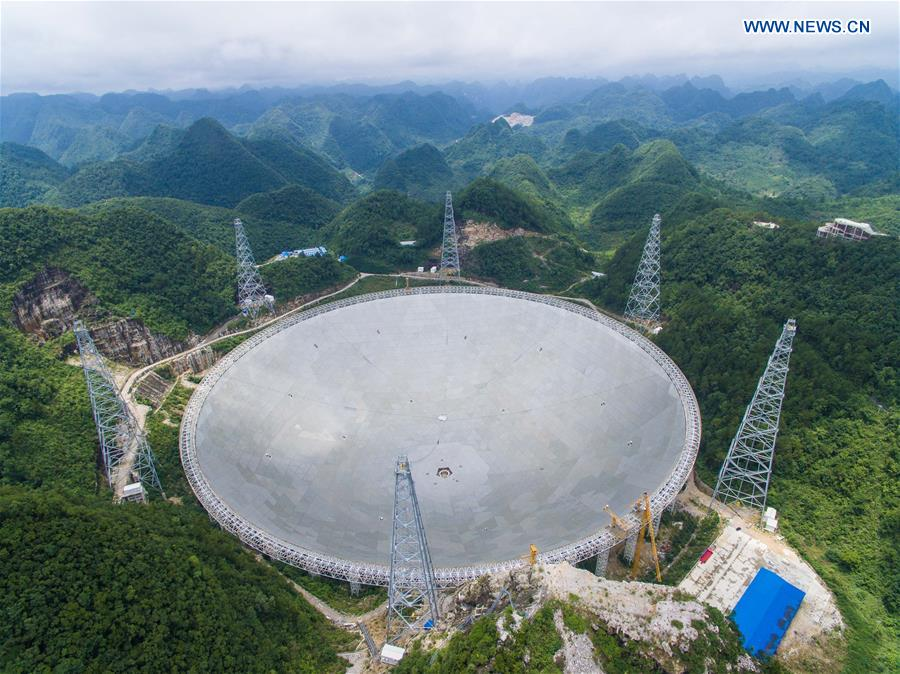
\includegraphics[width=.7\linewidth]{figs/photo_fast_dish.jpg}\\
\footnotesize Fig.~2. 500~m diameter parabolic antenna (FAST, China).
\vspace{3pt}
\begin{itemize}
  \footnotesize
  \item Resolution depends on antenna \textbf{aperture} (biggest today
  $\approx500$~m).
  \item Cost: \textbf{millions of dollars} of infrastructure.
\end{itemize}
\column{.48\textwidth}
\centering
\textbf{Aperture Synthesis}\\{\footnotesize (New concept)}\\[3pt]
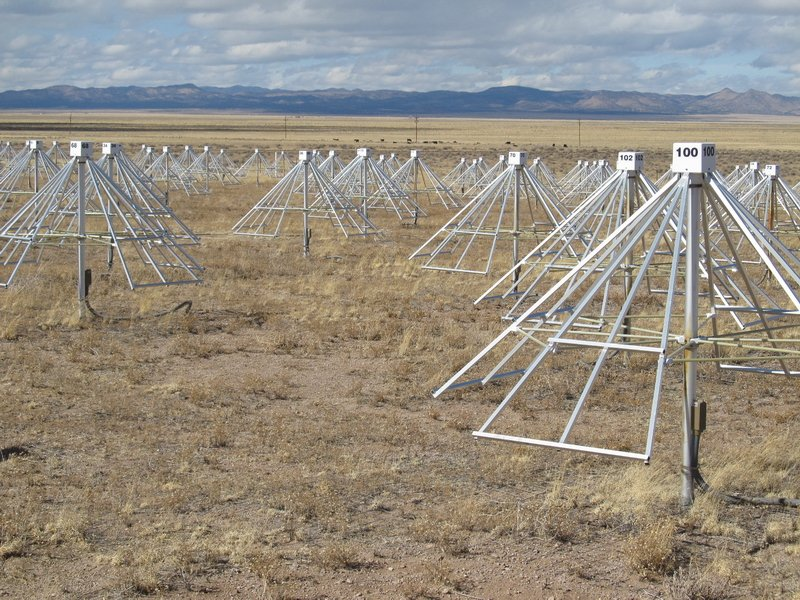
\includegraphics[width=.7\linewidth]{figs/photo_dlite_array.jpg}\\
\footnotesize Fig.~3. DLITE station in the USA, 32 LWA antennas.
\vspace{3pt}
\begin{itemize}
  \footnotesize
  \item Resolution depends on the biggest \textbf{baseline} between
  antennas (thousands of m).
  \item Cost scales with antenna count --- \textbf{thousands of
  dollars} each, many frequencies possible.
\end{itemize}
\end{columns}
\end{frame}

\begin{frame}{\ftitle{Field Trial: An Unexplained Result}}
\begin{columns}[c]
\column{.44\textwidth}
\textbf{Previous physical deployment}
\begin{itemize}
  \small
  \item Result: only an \textbf{ambiguous day/night trend} --- no clear
  interference fringes.
  \item Four candidate causes:
\end{itemize}
\begin{itemize}
  \footnotesize
  \item[$\square$] Phase-incoherent SDR oscillators?
  \item[$\square$] Cable insertion loss?
  \item[$\square$] Local RFI?
  \item[$\square$] Thermal noise floor too high?
\end{itemize}
\column{.5\textwidth}
\centering
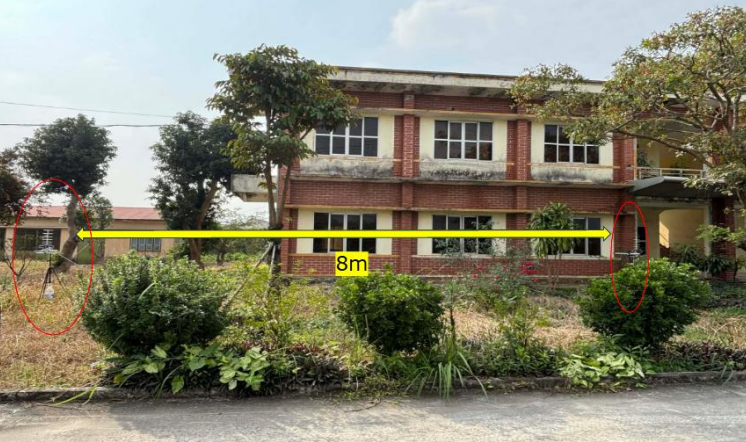
\includegraphics[width=\linewidth]{figs/photo_xuan_mai_field.png}\\
\small Fig.~4. Xuan Mai field trial: 2-element Yagi-Uda, 8~m baseline.
\end{columns}
\vspace{6pt}
\begin{alertblock}{Insight}
\small A hardware chain system cannot be debugged by observing and fixing
it blindly. We must build a physically grounded simulation to separate
and quantify these effects \textbf{before} further expensive hardware
deployment.
\end{alertblock}
\end{frame}

\begin{frame}{\ftitle{Objectives}}
\centering
\textbf{This thesis came out to answer two main ideas}
\vspace{10pt}

\begin{columns}[t]
\column{.48\textwidth}
\begin{block}{Build a trustworthy physics simulation}
\centering
\footnotesize Signal $\to$ correlator $\to$ image. Validated against
classical theory and real hardware, so it can safely stand in before
expensive field testing.
\end{block}
\column{.48\textwidth}
\begin{block}{Optimize antenna placement (array geometry)}
\centering
\footnotesize Use that simulator to search many array layouts. Find
which placement of the same antennas gives the best 2-D resolution,
without buying more hardware.
\end{block}
\end{columns}
\end{frame}

% ============================================================
\section{Theoretical Background}

\begin{frame}{\ftitle{Roadmap: The Problem, End to End}}
\centering
\scalebox{0.88}{%
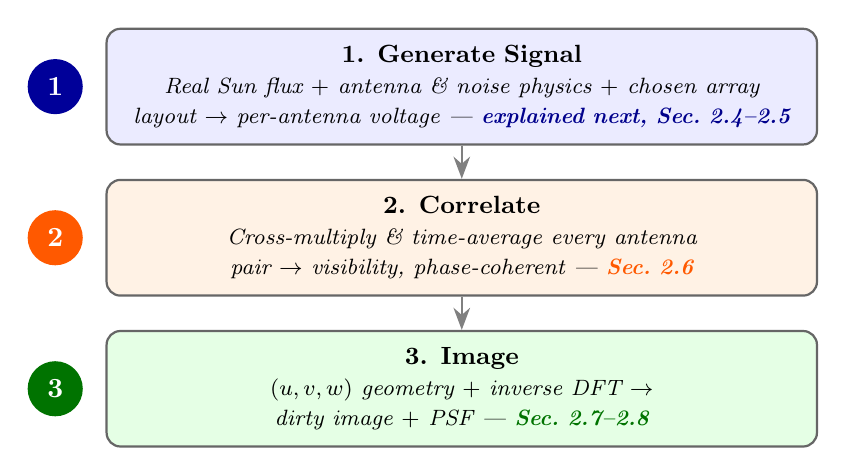
\begin{tikzpicture}[
  badge/.style={circle, fill=blue!60!black, text=white, font=\bfseries,
                minimum size=0.7cm, inner sep=0pt},
  proc/.style={rectangle, rounded corners=5pt, draw=black!60, thick,
               text width=8.6cm, align=center, inner sep=6pt,
               minimum height=1.15cm, font=\small},
  arr/.style={-{Stealth[length=8pt]}, thick, black!50}
]
\node[proc, fill=blue!8] (gen) {\textbf{1. Generate Signal}\\{\footnotesize\itshape
Real Sun flux $+$ antenna \& noise physics $+$ chosen array layout
$\to$ per-antenna voltage --- \textcolor{blue!55!black}{\textbf{explained next, Sec.~2.4--2.5}}}};
\node[badge, left=8pt of gen] {1};
\node[proc, fill=orange!10, below=12pt of gen] (corr) {\textbf{2. Correlate}\\{\footnotesize\itshape
Cross-multiply \& time-average every antenna pair $\to$ visibility, phase-coherent
--- \textcolor{orange!70!red}{\textbf{Sec.~2.6}}}};
\node[badge, fill=orange!70!red, left=8pt of corr] {2};
\node[proc, fill=green!10, below=12pt of corr] (img) {\textbf{3. Image}\\{\footnotesize\itshape
$(u,v,w)$ geometry $+$ inverse DFT $\to$ dirty image $+$ PSF
--- \textcolor{green!45!black}{\textbf{Sec.~2.7--2.8}}}};
\node[badge, fill=green!45!black, left=8pt of img] {3};
\draw[arr] (gen) -- (corr);
\draw[arr] (corr) -- (img);
\end{tikzpicture}%
}

\vspace{6pt}
\small $\Rightarrow$ Once this chain is trustworthy, the \textbf{same three
boxes} are re-run for every candidate antenna layout --- comparing those
outputs is the second half of the thesis (Chapter~5).
\end{frame}

\begin{frame}{\ftitle{Solar Radio Bursts: Types I--V}}
\begin{columns}[c]
\column{.55\textwidth}
\begin{itemize}
  \footnotesize
  \item Superimposed on the quiet-Sun thermal background, transient bursts can
  raise the flux by \textbf{orders of magnitude}.
  \item \textbf{Type I}: long-lived, narrowband noise storms.
  \item \textbf{Type III}: fast-drifting, electron beams on open field lines
  --- dominant at decimetre wavelengths.
  \item \textbf{Type II}: slowly drifting, traces coronal shock fronts (CMEs).
  \item \textbf{Type IV}: broadband continuum following flares.
  \item \textbf{Type V}: brief continuum sometimes following Type~III
  bursts, tracing trapped electron streams.
\end{itemize}
\column{.45\textwidth}
\centering
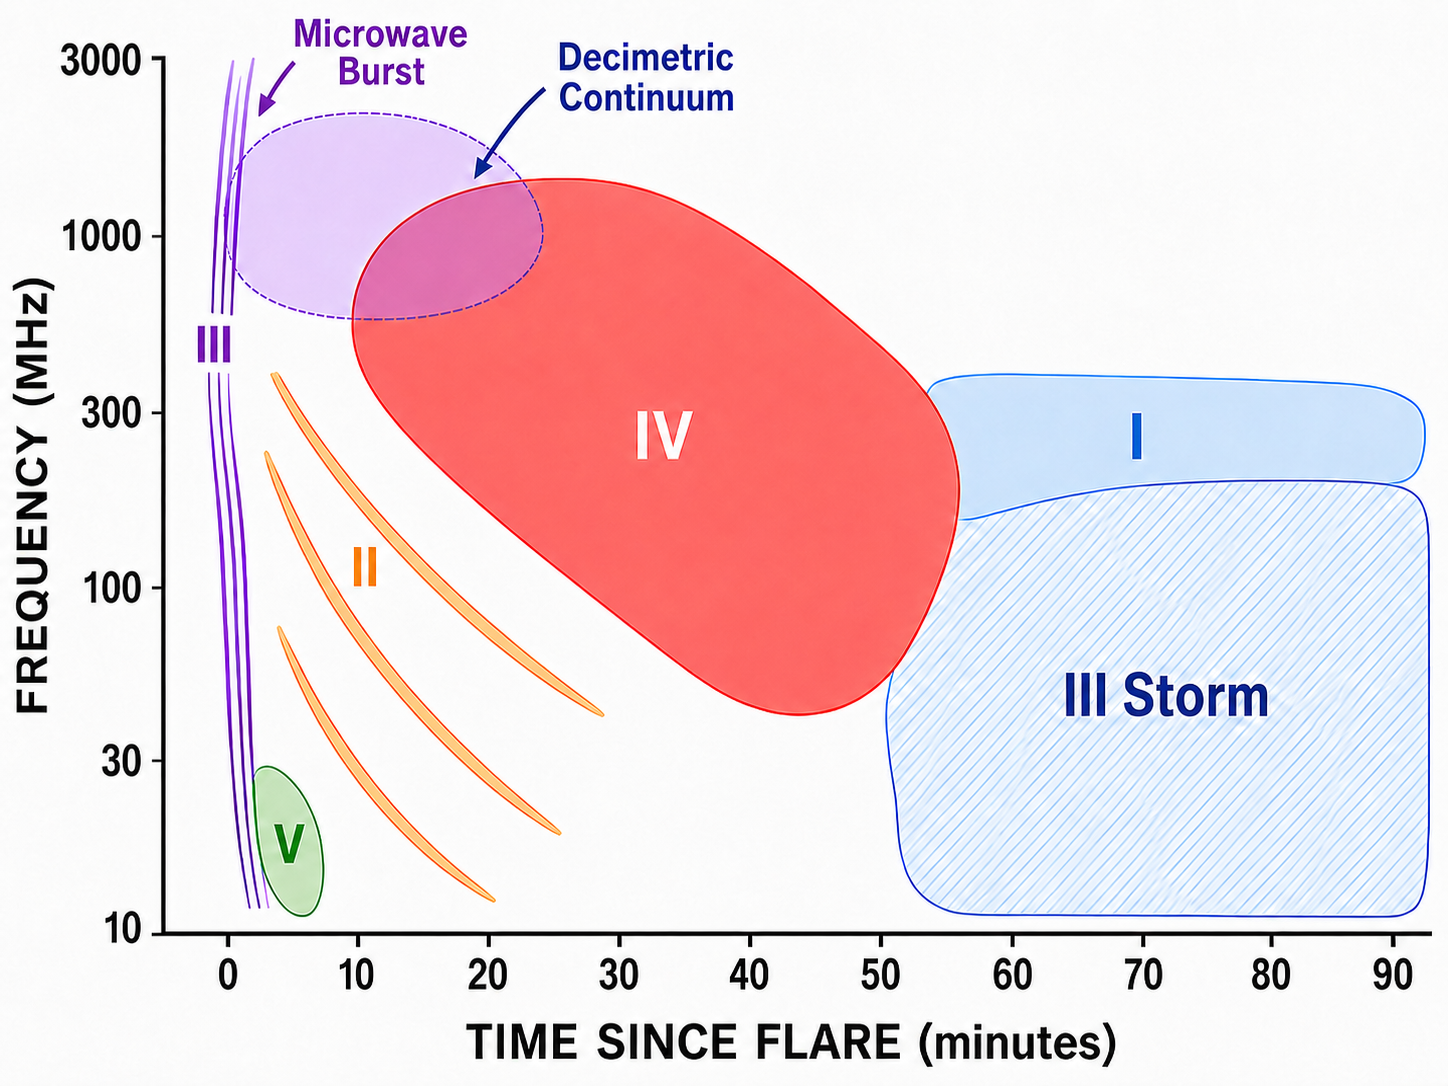
\includegraphics[width=\linewidth]{figs/fig_solar_dynamic_spectrum.png}
\end{columns}
\vspace{4pt}
\small Adapted from McLean \& Labrum and Dulk~\cite{dulk1985}.
\end{frame}

\begin{frame}{\ftitle{The Idea of Interferometry: Why Many Antennas?}}
\centering
\setlength{\tabcolsep}{2pt}
\begin{tabular}{ccc}
\parbox{.3\linewidth}{\centering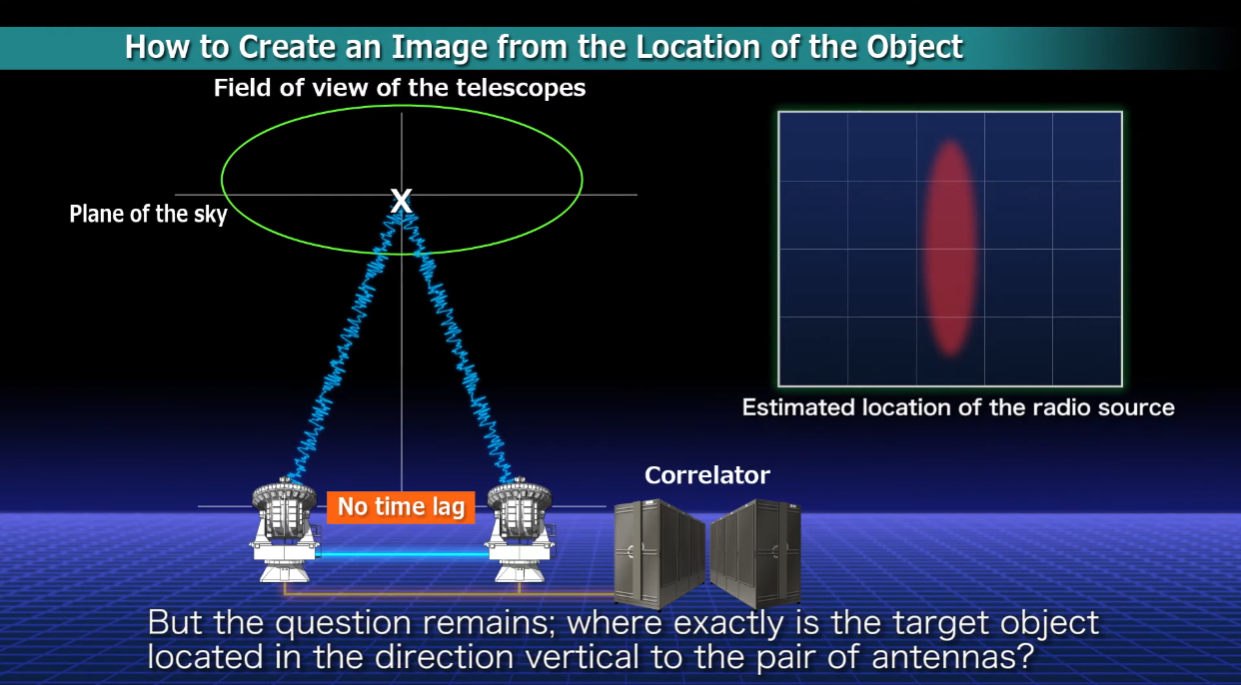
\includegraphics[width=\linewidth]{figs/fig_interf_1_notimelag.png}\\[2pt]\scriptsize 1. Two antennas, source dead ahead: no time lag.} &
\parbox{.3\linewidth}{\centering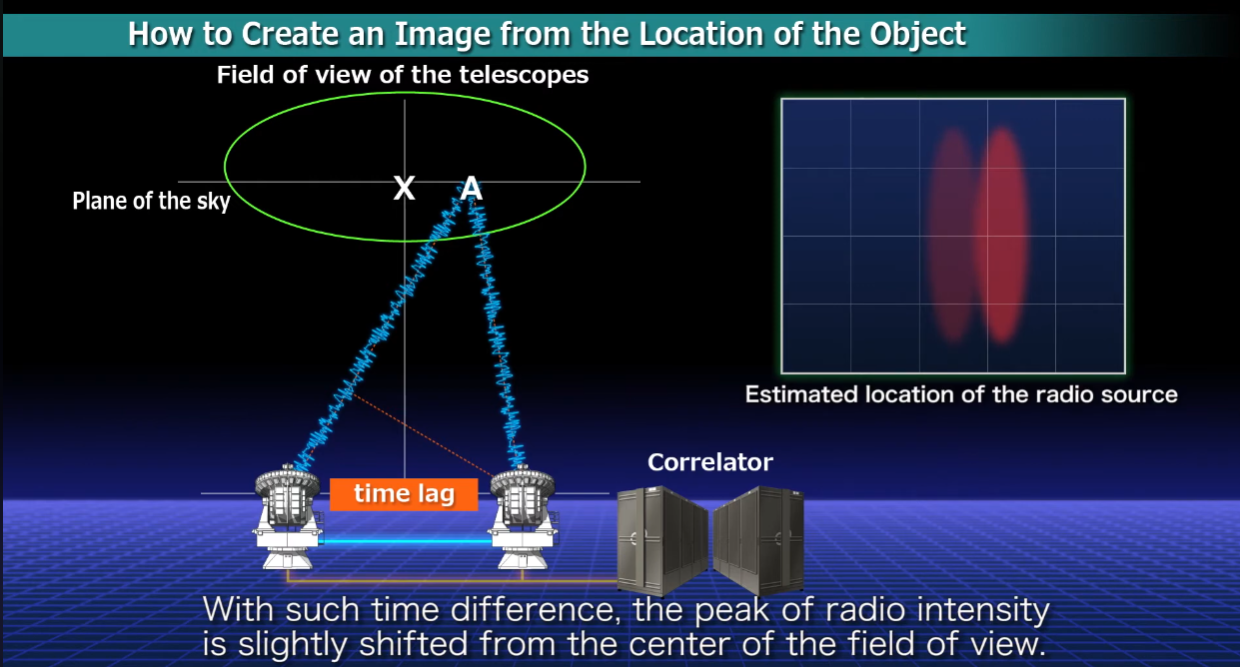
\includegraphics[width=\linewidth]{figs/fig_interf_2_timelag.png}\\[2pt]\scriptsize 2. Source off to one side: a tiny time lag appears.} &
\parbox{.3\linewidth}{\centering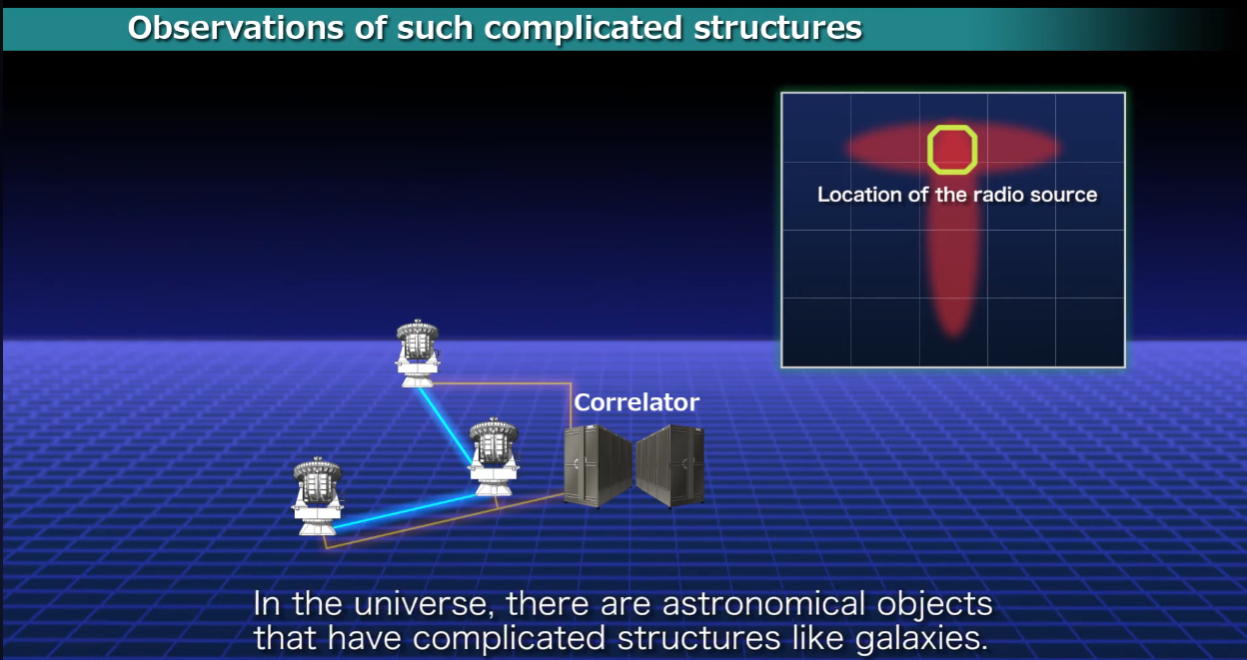
\includegraphics[width=\linewidth]{figs/fig_interf_3_threeant.png}\\[2pt]\scriptsize 3. A real source isn't one point --- need more.} \\[8pt]
\parbox{.3\linewidth}{\centering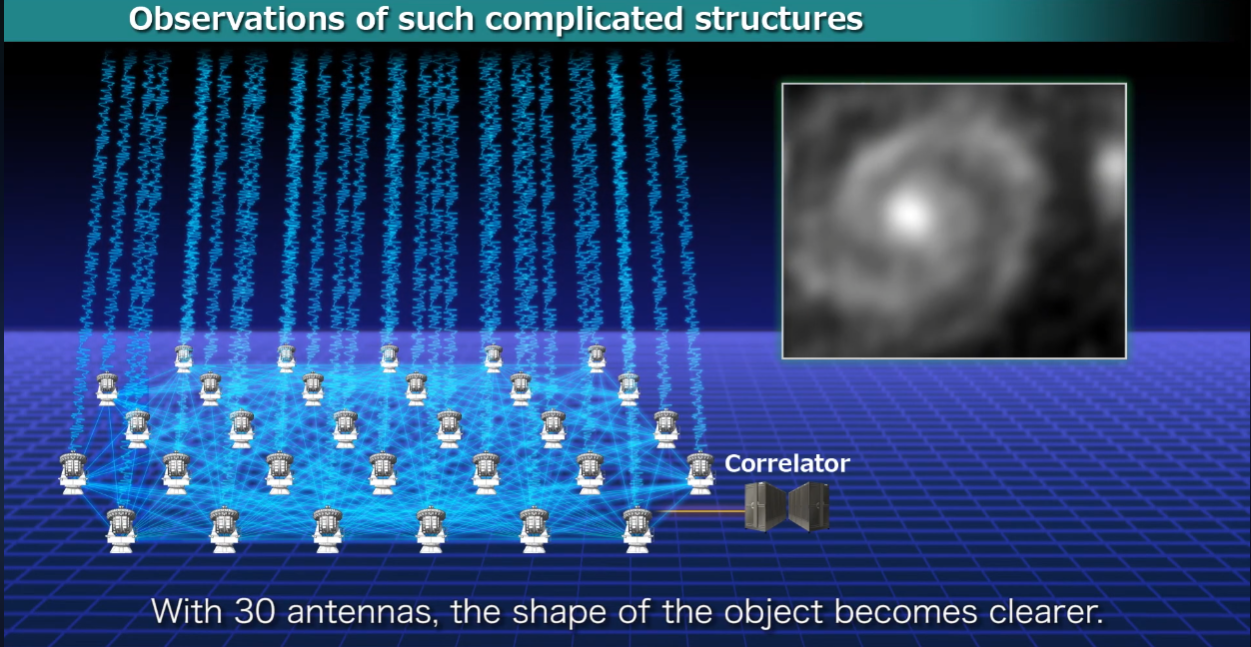
\includegraphics[width=\linewidth]{figs/fig_interf_5_30ant.png}\\[2pt]\scriptsize 5. With 30 antennas, the shape becomes clear.} &
\parbox{.3\linewidth}{\centering\Large$\Longleftarrow$} &
\parbox{.3\linewidth}{\centering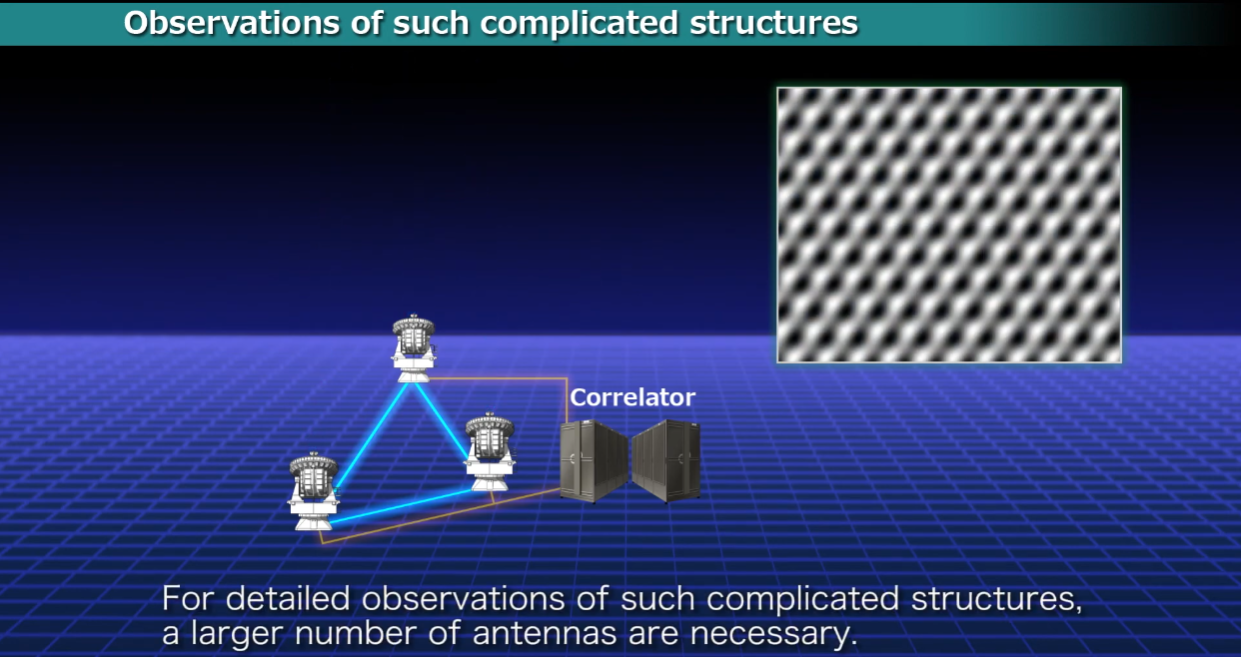
\includegraphics[width=\linewidth]{figs/fig_interf_4_fringepattern.png}\\[2pt]\scriptsize 4. Just 3 antennas: only a coarse, striped pattern.}
\end{tabular}
\vspace{4pt}

\small Each pair of antennas measures one time lag $\Rightarrow$ one
piece of the picture. \textbf{More antennas, more pairs, sharper image.}
\end{frame}

\begin{frame}{\ftitle{Key Formula 1: From Flux to Voltage (Friis)}}
\begin{flushright}
\scriptsize\colorbox{blue!12}{\textcolor{blue!55!black}{\textbf{Pipeline
Stage 1: Generate Signal}}}
\end{flushright}
\vspace{-6pt}
\textbf{Wavelength:} $\lambda = c/f \approx 0.49$~m at 610~MHz.
\vspace{6pt}

\textbf{Friis reception relation:}
\[
P_{\rm sig} = \tfrac{1}{2} A_e\, S_\nu\, \Delta\nu, \qquad A_e = \frac{\lambda^2 G}{4\pi}
\]
\begin{itemize}
  \item $S_\nu$: how much power the Sun sends per area (solar flux units,
  sfu)~\cite{friis1946}
  \item $A_e$: how much of that power one antenna can collect, from its
  simulated gain $G$
  \item Turn the received power into a voltage the receiver can read:
  $V_{\rm rms} = \sqrt{P_{\rm rx} R_{\rm load}}$
  \item[$\Rightarrow$] First step of the simulation: real Sun flux goes
  in, one voltage per antenna comes out.
\end{itemize}
\end{frame}

\begin{frame}{\ftitle{Key Formula 2: Receiver Noise (Johnson--Nyquist)}}
\begin{flushright}
\scriptsize\colorbox{blue!12}{\textcolor{blue!55!black}{\textbf{Pipeline
Stage 1: Generate Signal}}}
\end{flushright}
\vspace{-6pt}
\textbf{Johnson-Nyquist thermal noise:}
\[
P_n = k_B\, T_{\rm sys}\, \Delta\nu
\]
\textbf{Radiometer equation:}
\[
\mathrm{SNR} \;\propto\; \sqrt{N_s} \;=\; \sqrt{\Delta\nu\,\tau}
\]
\vspace{-8pt}
\begin{center}
\begin{block}{Symbols}
\centering\footnotesize
\begin{tabular}{rlrl}
$P_n$          & noise power            & $N_s$    & number of samples \\
$k_B$          & Boltzmann's constant   & $\tau$   & integration time \\
$T_{\rm sys}$  & system temperature     & $\Delta\nu$ & bandwidth \\
\end{tabular}
\end{block}
\end{center}
\vspace{-6pt}
\small $\Rightarrow$ This noise is added on top of the Friis voltage,
antenna by antenna, \textbf{before} anything is correlated.
\end{frame}

\begin{frame}{\ftitle{Key Formula 3: Correlator \& van Cittert--Zernike}}
\begin{flushright}
\scriptsize\colorbox{blue!12}{\textcolor{blue!55!black}{\textbf{Pipeline
Stage 2: Correlate}}}
\end{flushright}
\vspace{-6pt}
\centering
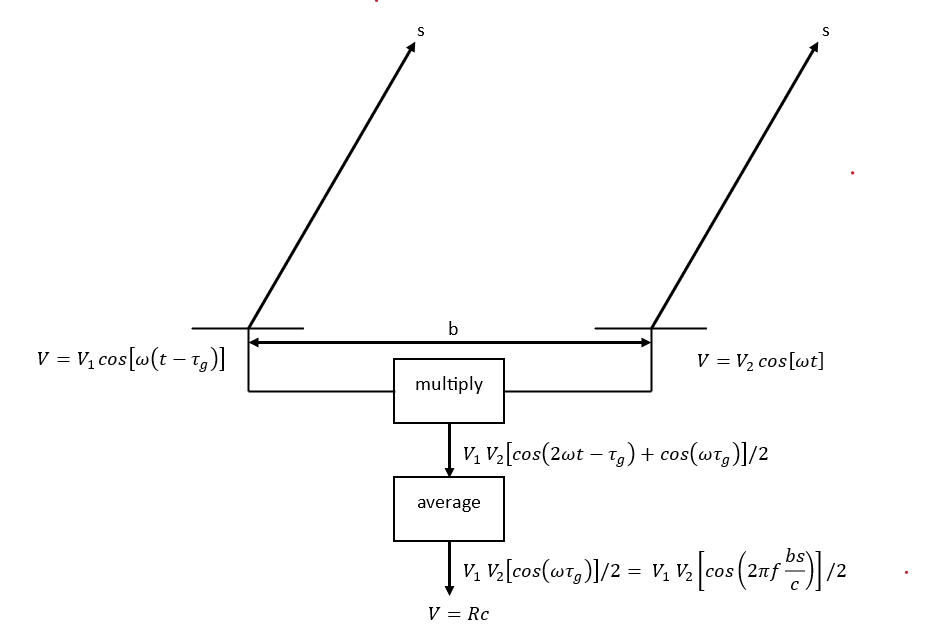
\includegraphics[width=0.6\linewidth]{figs/fig_correlator_multiply.png}

\vspace{6pt}
\footnotesize
Two antennas see the same wavefront with a time lag $\tau_g = B\sin\theta/c$
set by the baseline $B$. The \textbf{correlator} multiplies the two voltages
and averages: the result collapses to a single number, the
\textbf{visibility} $V \propto V_1V_2\cos(\omega\tau_g)$, that oscillates as
Earth's rotation sweeps $\theta$ --- a measurable \textbf{fringe}. Van
Cittert--Zernike: this fringe pattern $V(u,v)$ \emph{is} the Fourier
transform of the sky brightness $I(l,m)$.
\end{frame}

\begin{frame}{\ftitle{From Antenna Position to $(u,v,w)$}}
\begin{flushright}
\scriptsize\colorbox{blue!12}{\textcolor{blue!55!black}{\textbf{Pipeline
Stages 1 \& 3: Geometry}}}
\end{flushright}
\vspace{-6pt}
\textbf{Step 1 --- local to equatorial} (rotate by site latitude $\varphi$):
\[
\begin{pmatrix}X\\Y\\Z\end{pmatrix} =
\begin{pmatrix}
-\sin\varphi & 0 & \cos\varphi\\
0 & 1 & 0\\
\cos\varphi & 0 & \sin\varphi
\end{pmatrix}
\begin{pmatrix}E\\N\\U\end{pmatrix}
\]
\textbf{Step 2 --- equatorial to baseline} (rotate by hour angle $H$,
declination $\delta$):
\[
\begin{pmatrix}u\\v\\w\end{pmatrix} =
\begin{pmatrix}
\sin H & \cos H & 0\\
-\sin\delta\cos H & \sin\delta\sin H & \cos\delta\\
\cos\delta\cos H & -\cos\delta\sin H & \sin\delta
\end{pmatrix}
\begin{pmatrix}X\\Y\\Z\end{pmatrix}
\]
\begin{itemize}
  \footnotesize
  \item Same ground positions (East-North-Up), rotated first by \textbf{where
  the array sits} on Earth ($\varphi$), then by \textbf{where the Sun is
  right now} ($H,\delta$)~\cite{tms2017}.
  \item[$\Rightarrow$] One matrix, reused everywhere: per-antenna phase
  (Stage~1) and baseline coordinates for every antenna pair (Stage~3). As
  $H$ changes through the day, each baseline traces an arc in $(u,v)$.
\end{itemize}
\end{frame}

\begin{frame}{\ftitle{Aperture Synthesis Imaging}}
\begin{flushright}
\scriptsize\colorbox{blue!12}{\textcolor{blue!55!black}{\textbf{Pipeline
Stage 3: Image}}}
\end{flushright}
\vspace{-6pt}
\begin{itemize}
  \item $(u,v,w)$: every baseline, measured in wavelengths, as the Earth's
  rotation sweeps it through the sky.
  \item Fourier-transforming all the sampled visibilities gives the
  \textbf{dirty image}:
  \[
    I^{D} = I^{\rm sky} \ast B^{D}
  \]
  where $B^D$ is the synthesised beam (point-spread function, PSF).
  \item More baselines, better spread out $\Rightarrow$ a narrower PSF and
  sharper image --- exactly what the five-panel picture earlier showed.
  \item[$\Rightarrow$] Friis, Johnson--Nyquist, and van Cittert--Zernike:
  these three formulas are the physics running at each stage of the
  simulation pipeline, shown next.
\end{itemize}
\end{frame}

% ============================================================
\section{Antenna Design}

\begin{frame}{\ftitle{Antenna: The Yagi-Uda Element}}
\begin{columns}[c]
\column{.48\textwidth}
\centering
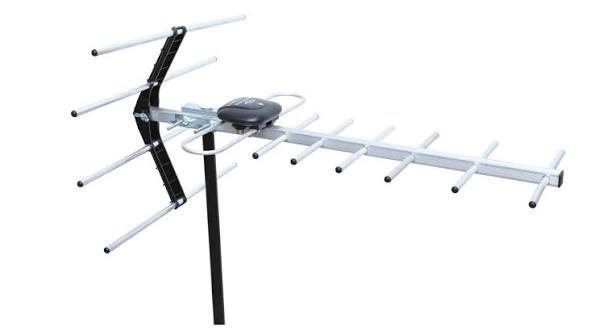
\includegraphics[width=\linewidth]{figs/photo_hkd_antenna.jpg}\\
\small Commercial HKD~G11KD-T2 Yagi-Uda: six directors, U-frame reflector.
\column{.48\textwidth}
\centering
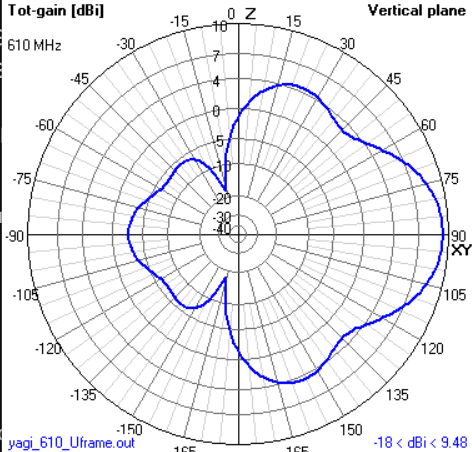
\includegraphics[width=\linewidth]{figs/fig_pattern_eplane_crop.png}\\
\small Simulated E-plane (vertical) pattern, 610~MHz (4NEC2).
\end{columns}
\vspace{4pt}
\begin{itemize}
  \footnotesize
  \item Low-cost, off-the-shelf UHF TV antenna, repurposed as a solar
  radio interferometer element.
  \item Directional gain toward the horizon --- well matched to a
  low-elevation solar transit at Learmonth's latitude.
\end{itemize}
\end{frame}

\begin{frame}{\ftitle{Yagi-Uda Antenna: 4NEC2 Model \& Performance}}
\begin{columns}[c]
\column{.46\textwidth}
\begin{table}
\footnotesize
\begin{tabular}{lc}
\toprule
\textbf{Quantity} & \textbf{Value} \\
\midrule
Input $Z$ & $108.4 - j22.0\;\Omega$ \\
Forward gain & 9.48 dBi \\
HPBW & $\approx 52^\circ$ \\
SWR (75~$\Omega$) & 1.55 \\
\bottomrule
\end{tabular}
\end{table}
\begin{itemize}
  \footnotesize
  \item Commercial folded-dipole Yagi-Uda (6 directors), modelled
  wire-by-wire in 4NEC2~\cite{nec2}.
  \item Real part close to 75~$\Omega$ coax $\Rightarrow$ good match
  without a balun network.
\end{itemize}
\column{.5\textwidth}
\centering
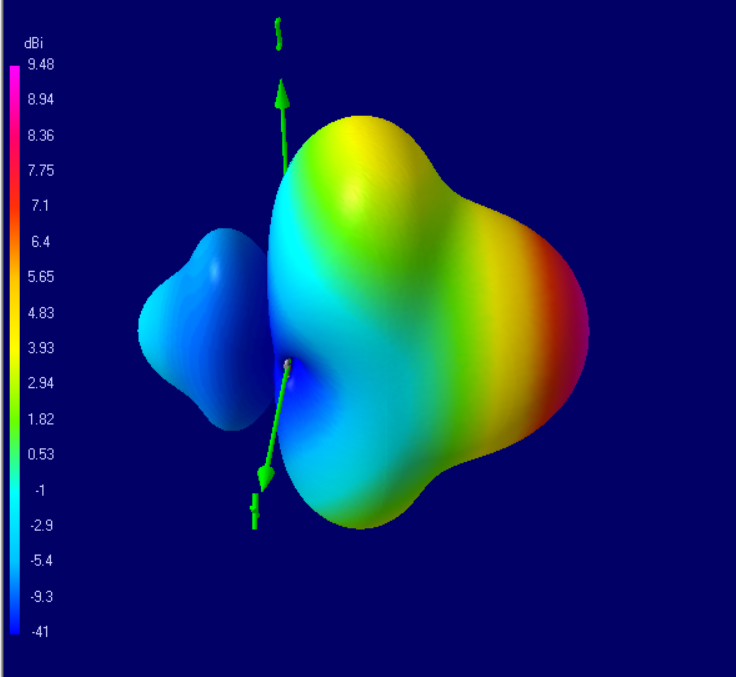
\includegraphics[width=\linewidth]{figs/fig_3d_radiation_pattern.png}\\
\small 3-D directivity pattern at 610~MHz.
\end{columns}
\end{frame}

% ============================================================
\section{Simulation Pipeline}

\begin{frame}{\ftitle{Simulation \& Antenna Input Parameters}}
\textbf{Table 1. Technical inputs for the simulation}
\begin{table}
\footnotesize
\centering
\begin{tabular}{ll}
\toprule
\textbf{Parameter} & \textbf{Value} \\
\midrule
Input source     & SWS Learmonth archived flux, 20 Mar 2025 \\
Frequency        & 610~MHz \\
Bandwidth        & 1~MHz \\
Baseline range   & 8~m to 130~m \\
Transient types  & Type~II, III, IV, and quiet Sun \\
Antenna          & Yagi-Uda commercial antenna \\
System temperature ($T_{\rm sys}$) & 150~K \\
Site latitude    & $-22.2^\circ$ (Learmonth) \\
Wavelength       & 0.49~m \\
\bottomrule
\end{tabular}
\end{table}
\vspace{2pt}
\textbf{Antenna input (from the 4NEC2 model, Section~3):}
\begin{itemize}
  \footnotesize
  \item Input impedance $108.4 - j22.0\;\Omega$, forward gain
  \textbf{9.48~dBi}, HPBW $\approx52^\circ$, SWR (75~$\Omega$) 1.55.
  \item[$\Rightarrow$] These two tables are the only numbers the
  simulator needs --- everything else is computed from them.
\end{itemize}
\end{frame}

\begin{frame}{\ftitle{Simulation Pipeline: From Flux to Image}}
\centering
\scalebox{0.92}{%
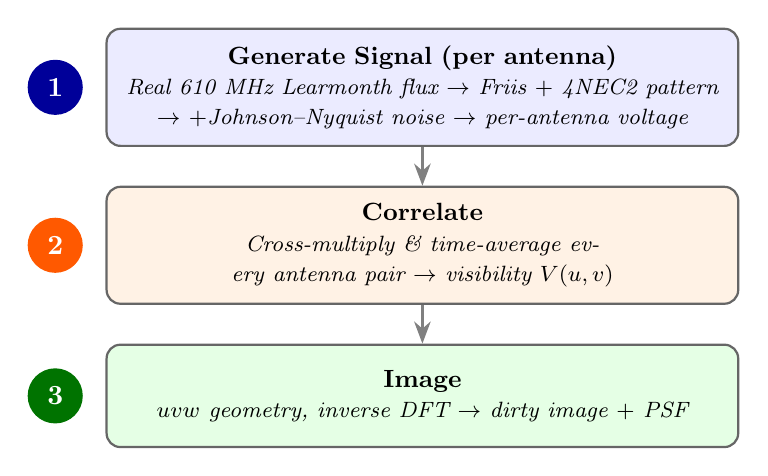
\begin{tikzpicture}[
  badge/.style={circle, fill=blue!60!black, text=white, font=\bfseries,
                minimum size=0.7cm, inner sep=0pt},
  proc/.style={rectangle, rounded corners=5pt, draw=black!60, thick,
               text width=7.6cm, align=center, inner sep=6pt,
               minimum height=1.3cm, font=\small},
  arr/.style={-{Stealth[length=8pt]}, thick, black!50}
]
\node[proc, fill=blue!8] (gen) {\textbf{Generate Signal (per antenna)}\\{\footnotesize\itshape Real 610~MHz Learmonth flux $\to$ Friis $+$ 4NEC2 pattern $\to$ $+$\mbox{Johnson--Nyquist} noise $\to$ per-antenna voltage}};
\node[badge, left=8pt of gen] {1};
\node[proc, fill=orange!10, below=14pt of gen] (corr) {\textbf{Correlate}\\{\footnotesize\itshape Cross-multiply \& time-average every antenna pair $\to$ visibility $V(u,v)$}};
\node[badge, fill=orange!70!red, left=8pt of corr] {2};
\node[proc, fill=green!10, below=14pt of corr] (img) {\textbf{Image}\\{\footnotesize\itshape $uvw$ geometry, inverse DFT $\to$ dirty image $+$ PSF}};
\node[badge, fill=green!45!black, left=8pt of img] {3};
\draw[arr] (gen) -- (corr);
\draw[arr] (corr) -- (img);
\end{tikzpicture}%
}

\vspace{4pt}
\footnotesize A second, faster analytic path (van Cittert--Zernike forward
visibility model) reuses the same geometry code to cross-check this chain
and to sweep array geometries quickly in Chapter~5.
\end{frame}

\begin{frame}{\ftitle{Input Data \& Voltage Synthesis}}
\centering
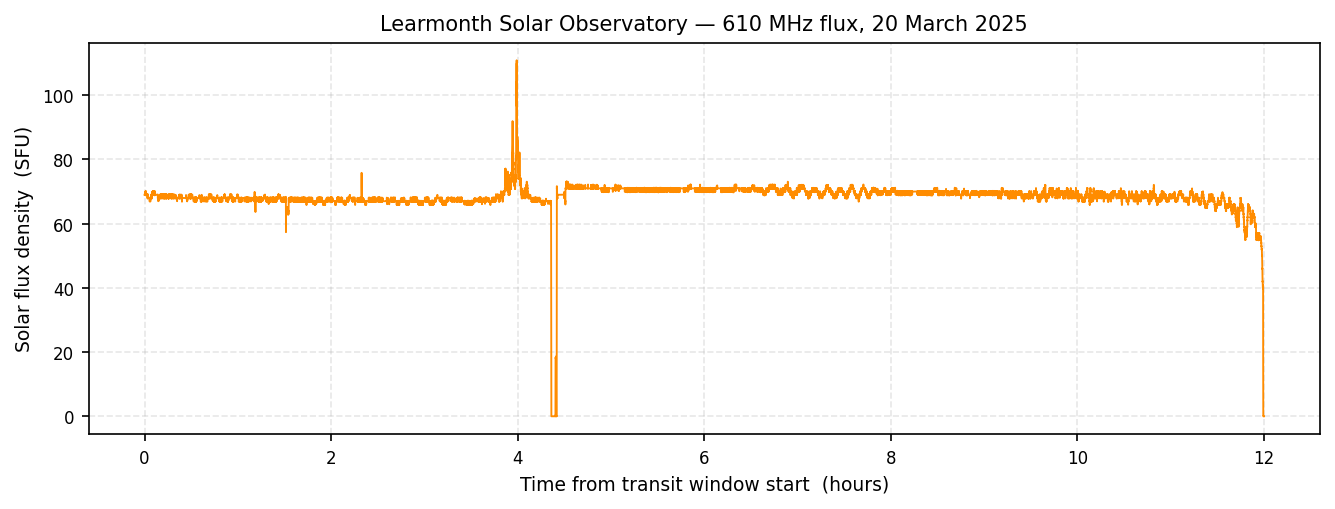
\includegraphics[width=0.58\linewidth]{figs/fig_sws_flux_day.png}\\[1pt]
{\scriptsize $\Downarrow$ Friis $+$ 4NEC2 pattern $+$ \mbox{Johnson--Nyquist} noise}\\[1pt]
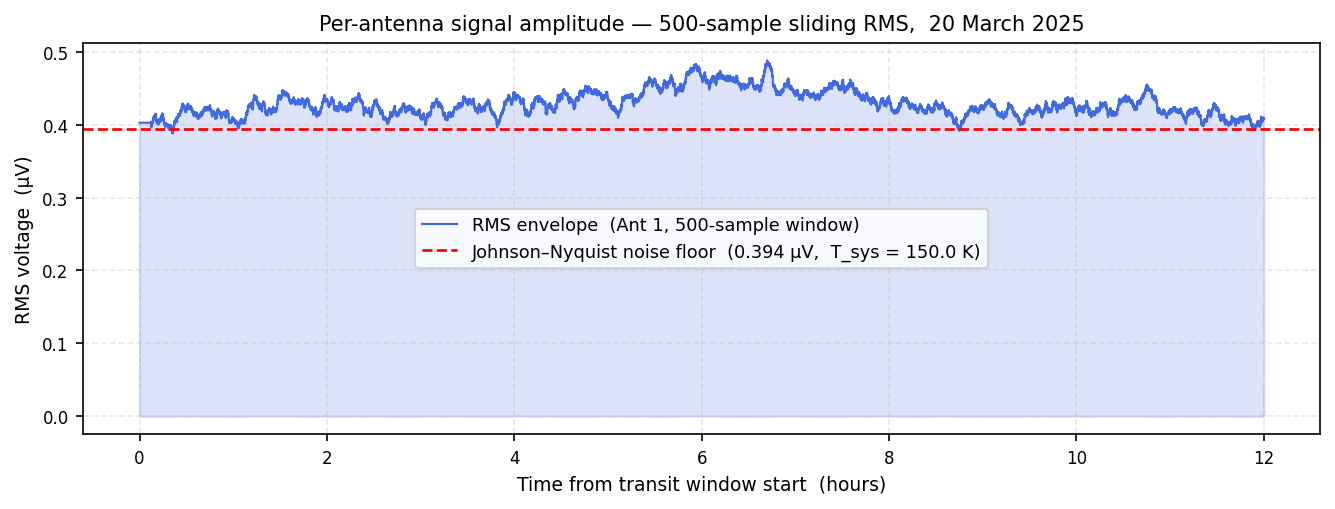
\includegraphics[width=0.58\linewidth]{figs/fig_voltage_env.png}

\vspace{1pt}
\begin{itemize}
  \footnotesize
  \item \textbf{Top:} real, archived, already-calibrated 610~MHz flux
  from SWS Learmonth, Australia~\cite{sws} (20 March 2025) --- the raw
  input, not re-simulated internally.
  \item \textbf{Bottom:} the same track after Friis power conversion,
  the 4NEC2 primary beam, and additive noise --- per-antenna complex
  baseband voltage, ready for correlation.
\end{itemize}
\end{frame}

\begin{frame}{\ftitle{Correlation: Visibility \& Phase Coherence}}
\begin{flushright}
\scriptsize\colorbox{blue!12}{\textcolor{blue!55!black}{\textbf{Pipeline
Stage 2: Correlate}}}
\end{flushright}
\vspace{-6pt}
\centering
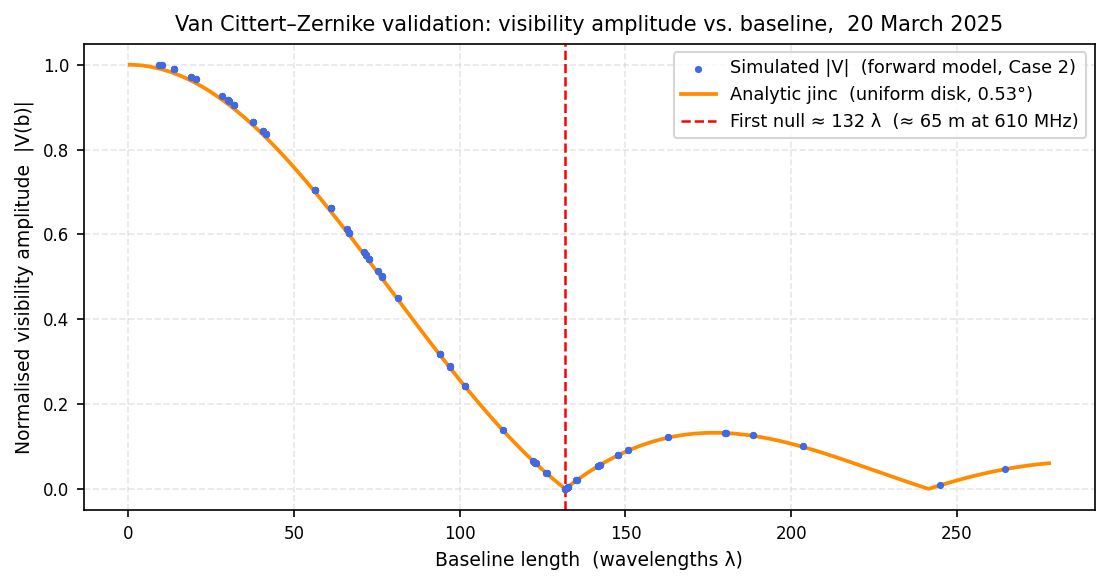
\includegraphics[width=0.62\linewidth]{figs/fig_visibility_jinc.png}

\vspace{4pt}
\begin{itemize}
  \footnotesize
  \item Every antenna pair is cross-multiplied and time-averaged into one
  complex number per baseline: the \textbf{visibility}
  $V(u,v) = |V|\,e^{j\phi}$.
  \item \textbf{Phase-coherent:} the two voltages stay locked in phase
  across the integration window --- this is what lets Earth's rotation
  build up the full $(u,v)$ plane (Earth-rotation synthesis).
  \item Output: one complex visibility per baseline per time sample, ready
  for imaging.
\end{itemize}
\end{frame}

\begin{frame}{\ftitle{Array Geometry: Site \& Observing Setup}}
\centering
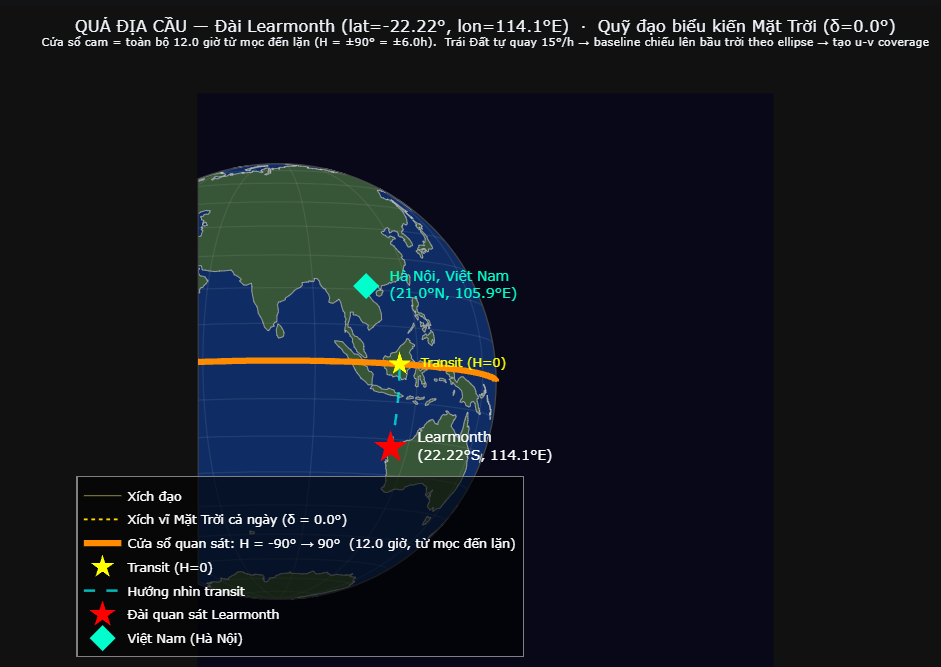
\includegraphics[width=0.62\linewidth]{figs/fig_globe_track.png}

\vspace{4pt}
\begin{itemize}
  \footnotesize
  \item Learmonth Observatory, site latitude $-22.2^\circ$; the Sun
  transits within hour angle $H\in[\pm90^\circ]$, a 12-hour observing
  window.
  \item This site geometry, plus each antenna's East-North-Up position,
  is exactly what feeds the $(u,v,w)$ transform (Section~2.7) --- the
  starting point for every array layout compared next.
\end{itemize}
\end{frame}

\begin{frame}{\ftitle{Imaging Validation: True Sky $\times$ PSF}}
\centering
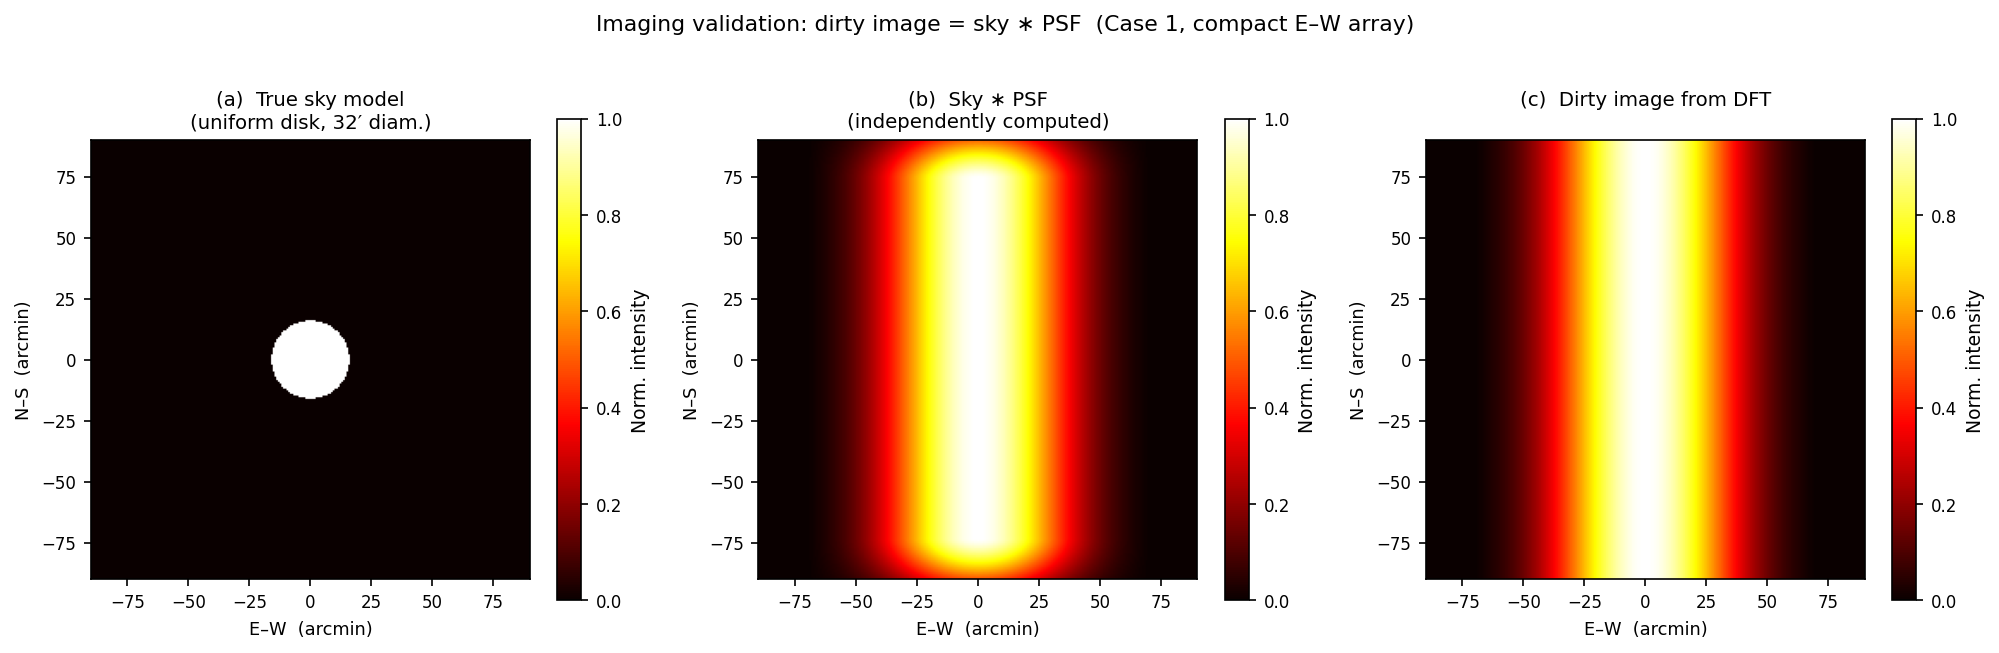
\includegraphics[width=\linewidth]{figs/fig_sky_conv_psf.png}

\footnotesize (a) true sky $\ast$ (b) PSF $=$ (c) dirty image, computed
independently via gridding + FFT --- (b) and (c) agree, validating the
imaging stage for \emph{any} 2-D array layout.
\end{frame}

% ============================================================
\section{Evaluation \& Results}

\begin{frame}{\ftitle{Mutual Coupling: Antennas Behave Independently}}
\begin{columns}[c]
\column{.44\textwidth}
\begin{table}
\footnotesize
\centering
\begin{tabular}{lcc}
\toprule
\textbf{Method} & \textbf{SWR} & \makecell{\textbf{Return}\\\textbf{loss}} \\
\midrule
NanoVNA & 1.59 & $\approx-12.8$~dB \\
4NEC2   & 1.55 & $\approx-13.3$~dB \\
\bottomrule
\end{tabular}
\end{table}
\begin{itemize}
  \footnotesize
  \item Measured and simulated impedance agree within a narrow range ---
  the simulated antenna pattern is trustworthy enough to drive the imaging
  pipeline.
\end{itemize}
\column{.52\textwidth}
\centering
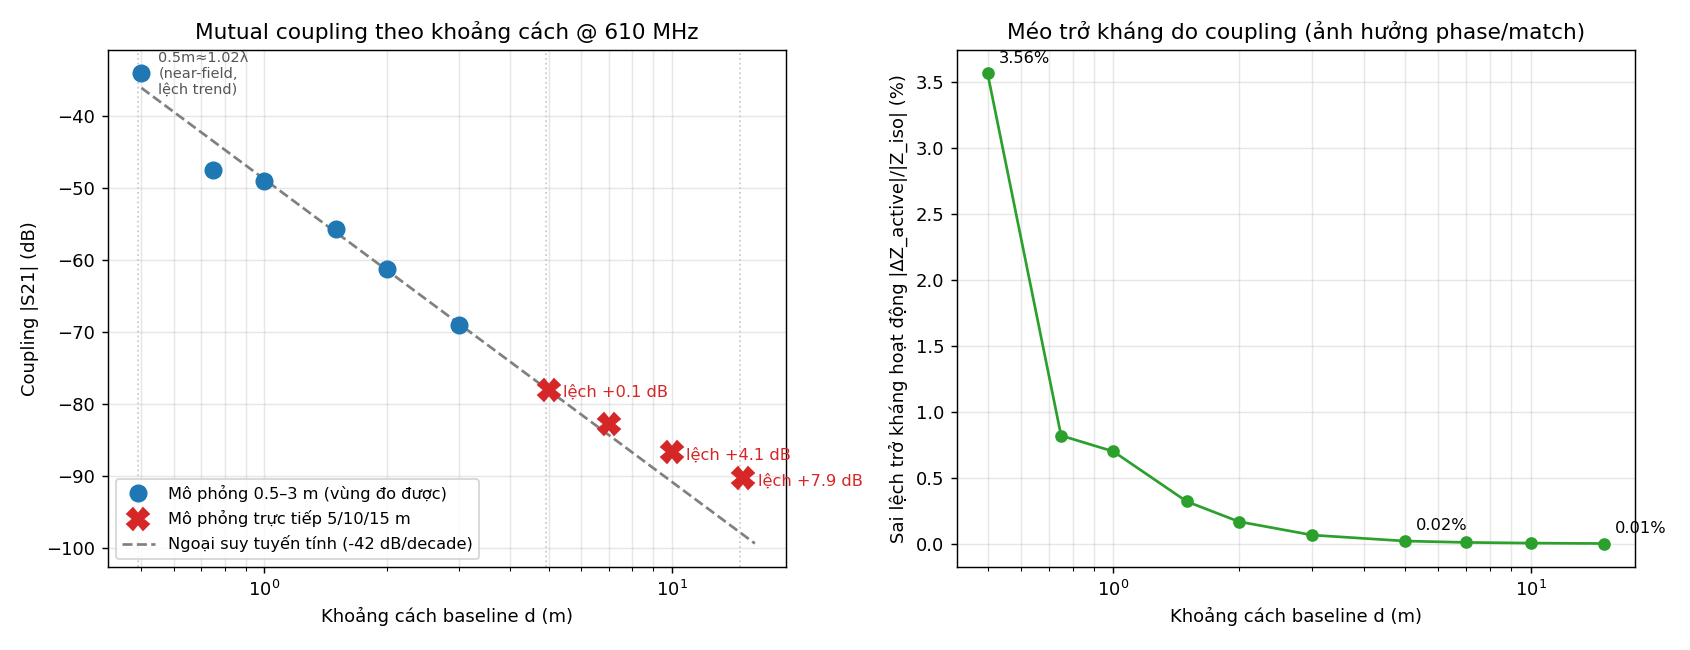
\includegraphics[width=\linewidth]{figs/fig_coupling_curve.png}
\begin{itemize}
  \footnotesize
  \item Coupling falls below $-78$~dB by 5~m and $-87$~dB by 10~m
  $\Rightarrow$ antennas behave as \textbf{independent sensors} at the
  operating baselines used in this thesis (8~m and above).
\end{itemize}
\end{columns}
\end{frame}

\begin{frame}{\ftitle{Visibility \& Fringe Pattern Validation}}
\begin{columns}[c]
\column{.5\textwidth}
\centering
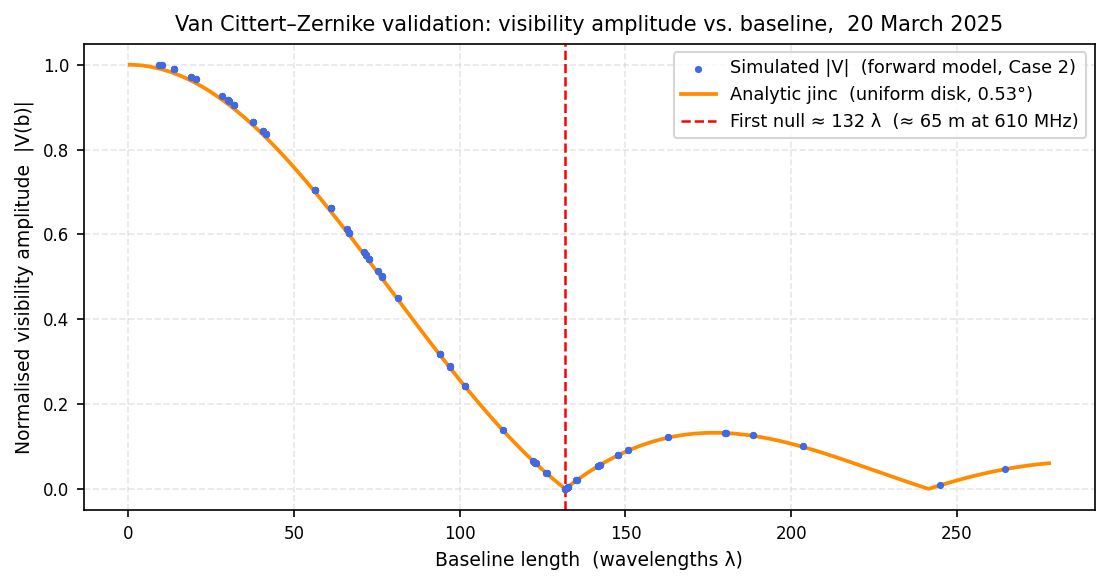
\includegraphics[width=\linewidth]{figs/fig_visibility_jinc.png}
\column{.5\textwidth}
\centering
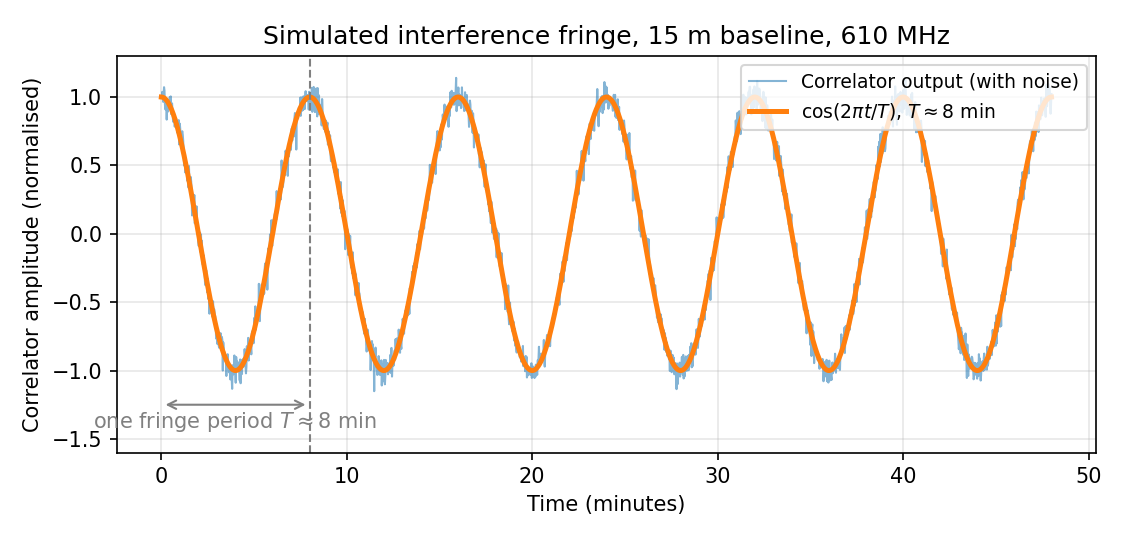
\includegraphics[width=\linewidth]{figs/fig_fringe_time_15m.png}
\end{columns}
\vspace{2pt}
\begin{itemize}
  \footnotesize
  \item \textbf{Left:} simulated visibility amplitude vs.\ baseline length
  falls right on the analytic jinc curve for a uniform solar disk, first
  null at $\approx130\,\lambda$ --- confirms the correlator implements van
  Cittert--Zernike correctly.
  \item \textbf{Right:} on a single 15~m baseline the correlator output
  oscillates with an $\approx$8-minute period, matching the analytic
  fringe-period prediction for that baseline and date.
  \item[$\Rightarrow$] Both independent checks agree with theory: the
  simulator can be trusted before comparing array layouts.
\end{itemize}
\end{frame}

\begin{frame}{\ftitle{Array Geometry Comparison}}
\centering
\scalebox{0.9}{%
\begin{minipage}{\linewidth}
\scriptsize
\renewcommand{\arraystretch}{1.0}
\setlength{\tabcolsep}{4pt}
\begin{tabular}{ccp{5.5cm}}
\toprule
\textbf{Layout} & \textbf{Dirty Image} & \textbf{Result} \\
\midrule
\parbox{1.3cm}{\centering
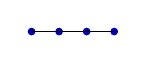
\begin{tikzpicture}[baseline=0pt]
\foreach \x in {0,0.35,0.7,1.05} \fill[blue!70!black] (\x,0) circle (1.4pt);
\draw[thin] (0,0) -- (1.05,0);
\end{tikzpicture}\\[1pt]{\tiny E-W line, 24~m}} &
\parbox{1.5cm}{\centering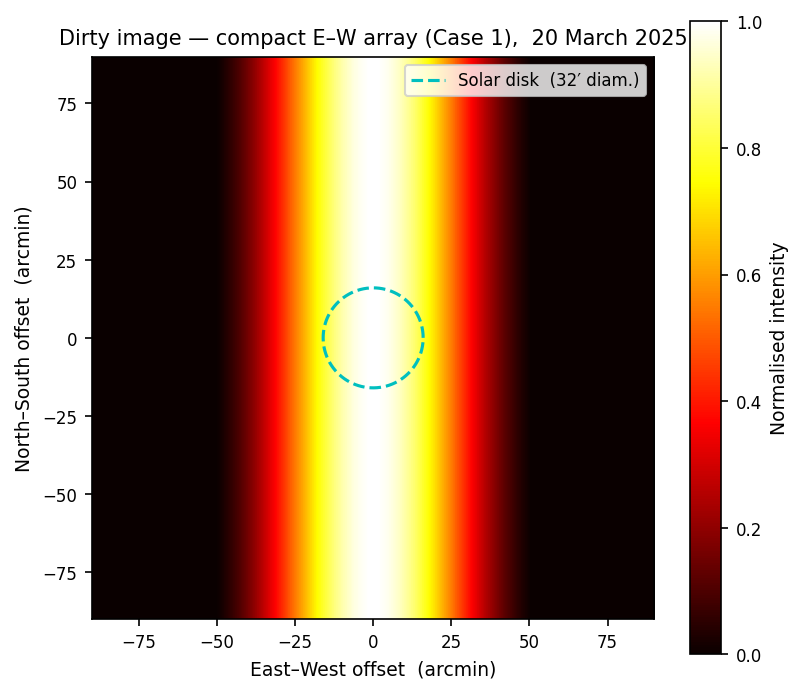
\includegraphics[width=\linewidth]{figs/fig_dirty_image.png}} &
\textbf{Case 1.} 1-D baselines only $\Rightarrow$ N-S FWHM $180.0'$ ---
smeared and unresolved in North-South. \\[1pt]

\parbox{1.3cm}{\centering
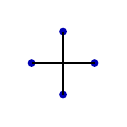
\begin{tikzpicture}[baseline=0pt]
\fill[blue!70!black] (0,0.4) circle (1.4pt);
\fill[blue!70!black] (0,-0.4) circle (1.4pt);
\fill[blue!70!black] (0.4,0) circle (1.4pt);
\fill[blue!70!black] (-0.4,0) circle (1.4pt);
\draw[thin] (0,0.4) -- (0,-0.4);
\draw[thin] (-0.4,0) -- (0.4,0);
\end{tikzpicture}\\[1pt]{\tiny Cross, 8~m}} &
\parbox{1.5cm}{\centering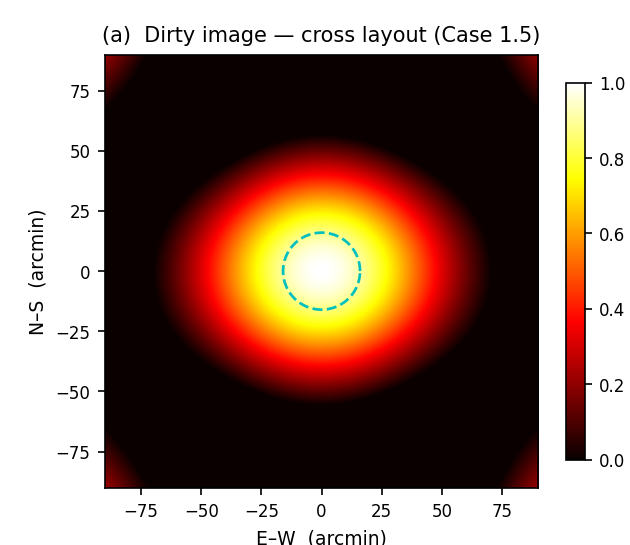
\includegraphics[width=\linewidth]{figs/fig_case15_dirty_crop.png}} &
\textbf{Case 1.5.} Same 4 antennas, adds a N-S arm $\Rightarrow$ N-S FWHM
$62.1'$ ($2.9\times$ better than Case~1). \\[1pt]

\parbox{1.3cm}{\centering
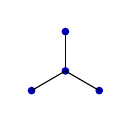
\begin{tikzpicture}[baseline=0pt]
\fill[blue!70!black] (0,0) circle (1.4pt);
\fill[blue!70!black] (0,0.5) circle (1.4pt);
\fill[blue!70!black] (0.43,-0.25) circle (1.4pt);
\fill[blue!70!black] (-0.43,-0.25) circle (1.4pt);
\draw[thin] (0,0) -- (0,0.5);
\draw[thin] (0,0) -- (0.43,-0.25);
\draw[thin] (0,0) -- (-0.43,-0.25);
\end{tikzpicture}\\[1pt]{\tiny Tri.+centre, 8~m}} &
\parbox{1.5cm}{\centering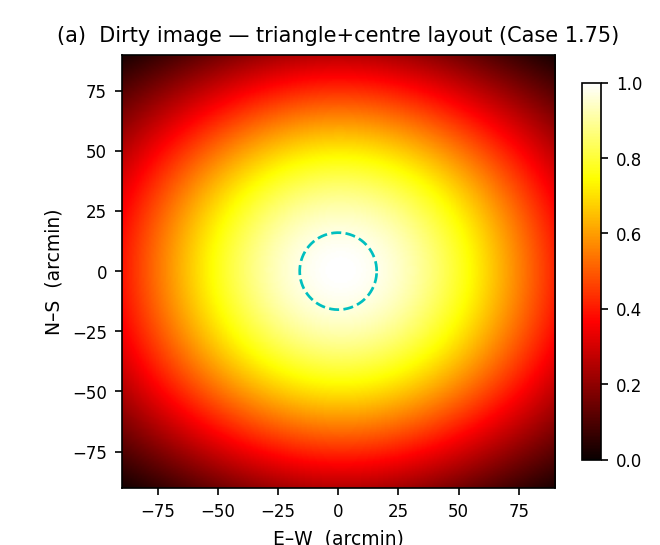
\includegraphics[width=\linewidth]{figs/fig_case175_dirty_crop.png}} &
\textbf{Case 1.75.} Same 4 antennas, DLITE-inspired triangle$+$centre~\cite{helmboldt2021dlite}: all 6 baselines point in distinct directions
$\Rightarrow$ N-S FWHM $19.8'$ ($\mathbf{9.1\times}$ better). \\[1pt]

\parbox{1.3cm}{\centering
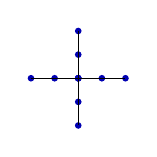
\begin{tikzpicture}[baseline=0pt]
\foreach \a in {0,0.3,0.6} {
  \fill[blue!70!black] (0,\a) circle (1.2pt);
  \fill[blue!70!black] (0,-\a) circle (1.2pt);
  \fill[blue!70!black] (\a,0) circle (1.2pt);
  \fill[blue!70!black] (-\a,0) circle (1.2pt);
}
\draw[thin] (0,0.6) -- (0,-0.6);
\draw[thin] (-0.6,0) -- (0.6,0);
\end{tikzpicture}\\[1pt]{\tiny Extended cross, 130~m}} &
\parbox{1.5cm}{\centering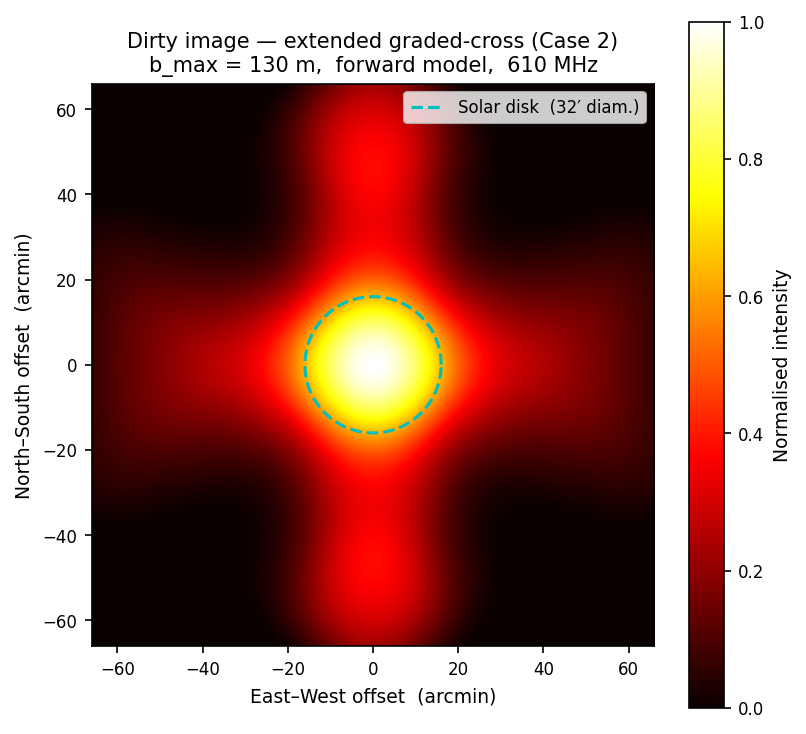
\includegraphics[width=\linewidth]{figs/fig_case2_image.png}} &
\textbf{Case 2.} Same antennas, spread out to 130~m baselines
$\Rightarrow$ E-W FWHM $\approx11'$ --- starts resolving the $32'$ solar
disk. \\
\bottomrule
\end{tabular}

\vspace{4pt}
\centering\normalsize\textbf{Same 4 antennas throughout --- placement, not
antenna count, is what improves resolution.}
\end{minipage}%
}
\end{frame}

% ============================================================
\section{Conclusion \& Future Work}

\begin{frame}{\ftitle{Objectives Revisited: Are We Done?}}
\begin{block}{\cmark\ 1. Build a trustworthy physics simulator}
\footnotesize
4NEC2 antenna model cross-checked against direct NanoVNA measurement;
mutual coupling confirms antennas act as independent sensors; simulated
visibility and fringe pattern match analytic van Cittert--Zernike theory
exactly.
\end{block}
\vspace{4pt}
\begin{block}{\cmark\ 2. Optimize antenna placement}
\footnotesize
Same 4-antenna hardware, four geometries tested: E-W line
$\to$ cross $\to$ DLITE-inspired triangle gives a
\textbf{9.1$\times$} N-S resolution gain from \emph{rearrangement alone};
extended cross (Case~2) begins resolving the $32'$ solar disk.
\end{block}
\vspace{4pt}
\begin{itemize}
  \footnotesize
  \item Bonus: a reproducible single-notebook workflow (raw flux $\to$
  calibrated dirty image, under two minutes) and a browser-based
  companion tool for live exploration.
\end{itemize}
\end{frame}

\begin{frame}{\ftitle{Conclusion \& Future Work}}
\begin{itemize}
  \item Space weather and GNSS impacts motivate ground-based solar radio
  monitoring; large dishes are costly, so low-cost interferometry (DLITE,
  and this work) is a realistic alternative.
  \item This thesis shows that a physically grounded, end-to-end
  simulation \emph{can} evaluate feasibility, signal chain, and array
  geometry \textbf{before} further hardware deployment --- turning the
  unexplained Xuan Mai field result into a concrete, testable design
  question.
\end{itemize}
\begin{block}{Future Work}
\footnotesize
\begin{itemize}
  \item FPGA hardware correlator, hardware-in-the-loop fringe validation.
  \item Physical DLITE-inspired array upgrade at Xuan Mai (triangle + centre).
  \item Recorded Type~II/III burst input; CLEAN
  deconvolution~\cite{hogbom1974}, multi-frequency imaging, real-time
  operation, GPS-disciplined clock.
\end{itemize}
\end{block}
\end{frame}

% ============================================================
\begin{frame}[allowframebreaks]
\frametitle{References}
\tiny{
\bibliography{refs_slides}
}
\end{frame}

\begin{frame}
\Huge{\centerline{Thank you!}}
\end{frame}

\end{document}
